\section{BitLocker Enabled}

Our final attack is against systems with \ac{BDE} using a \ac{TPM} 2.0, without additional \ac{PIN} or startup key, for key protection.
With this the Windows boot partition is encrypted, while the \ac{ESP} remains unencrypted, thus BitLocker does not affect the bootkit infection process.
When Secure Boot is enabled in combination with BitLocker, it has the same effect,s as observed in \autoref{sec:attacks:secure-boot}.
It also dictates which validation profile Windows uses to configure BitLocker, as mentioned in \autoref{sec:windows:security:bde}.
We perform our attack against both validation profiles, starting with \hyperref[tab:pcr-usage]{\code{\{0, 2, 4, 11\}}}.
This means either Secure Boot is disabled or \hyperlink{pcr7-binding}{\ac{PCR}7 is not bound}.

The validation profile \hyperref[tab:pcr-usage]{\code{\{7, 11\}}}, used when BitLocker uses Secure Boot for integrity validation, is covered in \autoref{sec:attacks:bitlocker:bitlocker-access-without-recovery-key}.

Due to the boot- and rootkit still sharing their core functionality we keep the approach abstract and refer to them with the expression \ac{UEFI} payload, not to be confused with our Windows payload that is deployed into the Windows installation.
We start by assuming that the infection is performed after BitLocker has already been fully set up, and cover the scenario that a user enables BitLocker while being infected at the end in \autoref{sec:attacks:bitlocker:bitlocker-access-without-recovery-key}.

\subsection{Infection}

When booting with our previous \ac{UEFI} payload, the \ac{NTFS} driver is unable to recognize any file system structure on the Windows boot partition, due to the \ac{FVE}.
This results in an inability to further deploy the Windows payload on the target system.
Additionally, during execution of the Windows Boot Manager, the BitLocker recovery prompt, shown in \autoref{fig:bitlocker-recovery-prompt}, interrupts the regular boot process requiring the drive's recovery key for decryption before being able to continue booting.
This happens due to \ac{TPM}'s \ac{PCR} values differing from what was initially used to seal the \ac{VMK}.
The rootkit is measured into \ac{PCR}0 and the bootkit into \ac{PCR}2.
This leaves the Windows bootloader unable to retrieve the unencrypted \ac{VMK} from the \ac{TPM} and as a result unable to decrypt the Windows installation \cite[Section 12]{windows-internals-7-part2}.

\begin{figure}[htb]
    \centering
    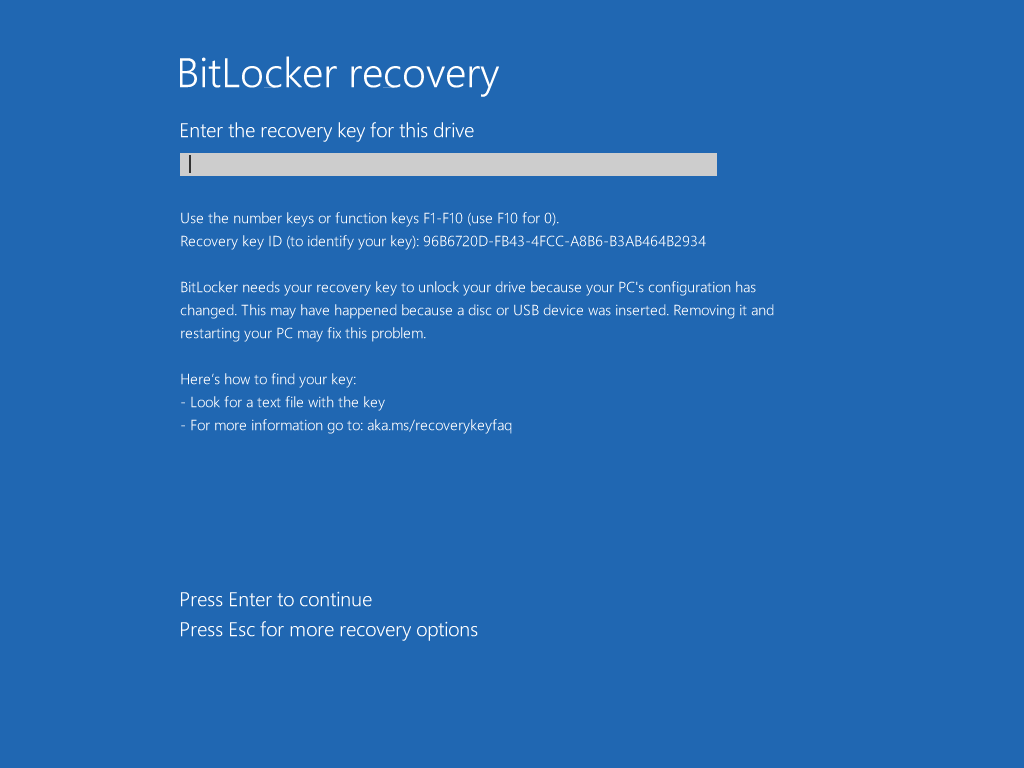
\includegraphics[width=1.0\textwidth]{attacks/bitlocker/bitlocker_recovery_prompt.png}
    \caption{BitLocker Recovery Prompt}
    \label{fig:bitlocker-recovery-prompt}
\end{figure}

BitLocker discovers the deviation in the boot flow, via the \ac{TPM} measurements, and blocks our \ac{UEFI} attack from accessing the Windows installation.
But how do users react to this?
After all it is asking them to enter their recovery key to resume the boot process and not to throw out their motherboard.
There are a few options for a user to proceed: they either trust the system and enter their recovery key, they mistrust the operating system, or they mistrust the entire system.
If they were to mistrust the whole system, they could take the hard drive out of the system and use the recovery key on a trusted system to recover data, being careful not to accidentally boot from the drive.
This would deny both our rootkit and bootkit any further access to any sensitive data.
If they were to mistrust the \ac{OS}, or they were to have neglected to properly back up their recovery key, they might perform a fresh installation of Windows.
In the case of our bootkit this would get rid of the threat, but the rootkit remains within the firmware image and would be part of the chain of trust for the fresh installation.

\subsection{BitLogger}

When the user enters their recovery key, the Windows Boot Manager uses the recovery key to decrypt the \ac{VMK} in the metadata entry that was encrypted using the recovery key when BitLocker was set up.
It then proceeds to access the BitLocked \ac{NTFS} drive containing the \program{Windload.efi} \ac{OS} loader.
This all still happens during the \ac{UEFI} boot environment, before \program{ExitBootServices} is called, as this is done within \program{Windload.efi}.
Unfortunately, we remain unable to access the Windows installation during this, as BitLocker only ever decrypts read operations in memory, leaving the drive fully encrypted at all times.
If we were to acquire the recovery key, we could use it to decrypt the \ac{VMK}, then the \ac{FVEK}, and in turn the drive ourselves.

This can be achieved by logging the keystrokes a user performs when they enter their recovery key into the recovery prompt.
Since the Windows Boot Manager is executed in the \ac{UEFI} boot environment, it has to use \ac{UEFI} protocols instead of the own Windows drivers to access the hardware.
This includes user input via the keyboard.
\ac{UEFI} offers two protocols for this purpose: the \nameref{lst:simple-text-input-protocol} and the \nameref{lst:simple-text-input-ex-protocol}.
We can quickly determine which of these is used by the Windows Boot manager by adding a simple \code{Print()} statement to the implementation in the \ac{EDK} II source code of the \ac{OVMF} image.
This change is also already enough to trigger the recovery prompt by invalidating the \ac{PCR} measurements.
A keystroke during the recovery prompt now shows us that the \nameref{lst:simple-text-input-ex-protocol} is being used.
The protocol structure is listed in \autoref{lst:simple-text-input-ex-protocol}.
The Windows Boot Manager uses the \code{ReadKeyStrokeEx()} function to retrieve the latest pending key press.
The protocol also offers the \code{WaitForKeyEx()} event, signaling when keystrokes are available.
Execution can be blocked until this event is emitted with the \code{WaitForEvent} boot service.
The protocol also allows users to register and unregister a callback function to react upon user input.
An exemplary use of the \code{ReadKeyStrokeEx()} is given below in \autoref{lst:handle-protocol-simple-text-input-ex}.

\vspace{1em}

\lstinputlisting[language=C,captionpos=b,label=lst:handle-protocol-simple-text-input-ex,firstline=7,caption={Example of using \code{HandleProtocol()} to retrieve an instance to the \nameref{lst:simple-text-input-ex-protocol} to use its \code{ReadKeyStrokeEx()} function to wait for and read a pending key press}]{code/handle_protocol_simple_text_input_ex.c}

We can intercept the \code{ReadKeyStrokeEx()} function call by using a technique called function hooking.
There are various ways of doing this, for example patching a jump instruction at the beginning of the target function to detour the execution flow.
\ac{UEFI} protocol hooking does not require such an invasive and processor architecture dependent technique.
When we take a closer look at how protocols are returned to their user we can see why.
The \ac{UEFI} boot services offer two functions, \code{HandleProtocol()} and \code{OpenProtocol()}, which can be used to retrieve a protocol instance.
\code{HandleProtocol()} is a simplified abstraction of \code{OpenProtocol()} and is implemented by the latter internally.
\code{OpenProtocol()} offers many additional options such exclusivity and notifying consumers when a protocol is being uninstalled \cite[Section 7.3]{uefi-spec}.

\autoref{lst:handle-protocol-simple-text-input-ex} shows how \code{HandleProtocol()} can be used to receive the \nameref{lst:simple-text-input-ex-protocol} instance installed on the active console input device \cite[Section 4.3]{uefi-spec}.
The input parameters are a device handle, the \ac{GUID} identifying the protocol and the address of a pointer to the protocol structure.
When calling \code{HandleProtocol()}, the value of the pointer is modified to point to the corresponding protocol instance.
The protocol instance itself is previously allocated by a driver and installed onto the device handle in \code{Start()} function of their \nameref{lst:driver-binding-protocol}.
The driver assigns the function fields with functions residing in the driver's image.
This is why it is important for a driver's image to remain loaded even after initial execution.
The important fact about this process is that a driver installs only one protocol instance per device handle and every protocol user receives the same address to the same protocol instance, given they use the same device handle.
The function interfaces of \code{HandleProtocol()} and \code{OpenProtocol()} would generally allow for the return of allocated memory containing a copy of the protocol's content, but the implementers of drivers, managing multiple devices, are encouraged to keep track of private data.
Private data is necessary to manage a device, but not part of the protocol interface.
The struct defining the private data contains the public protocol instance, so that it is possible to calculate address of the private data, using the protocol instance's address.
The protocol instance address is subtracted by the offset of the protocol within the private struct \cite[Section 8]{tianocore-edk2-driver-writer-s-guide}.
In \autoref{lst:private-data} we show an example of retrieving private data through the public protocol interface.
This keeps the protocol interface limited to the public functionality.
The \ac{UEFI} boot services are not aware of the size of the private data when managing protocol instances and therefor cannot make copies spanning the entire data.
On top of that, the private data likely contains information about the device state, as changes in the state would have to occur in each protocol user's instance to remain in a synchronous state.

\vspace{1em}

\lstinputlisting[language=C, captionpos=b, firstline=6, caption={Example of a driver using private data in the implementation of the \nameref{lst:disk-io-protocol}}, label=lst:private-data]{code/private_data.c}

Since our \ac{UEFI} payload is executed before the Windows Boot Manager, we can query all \nameref{lst:simple-text-input-ex-protocol} instances and change each function pointer of \code{ReadKeyStrokeEx()} to point to our function hook.
When the Windows Boot Manager later receives the protocol instance and calls \code{ReadKeyStrokeEx()} our hook is called instead of the original function.
The hook has to be implemented in memory, that remains loaded until the Windows Boot Manager uses \code{ReadKeyStrokeEx()}.
We can do this using a boot driver, as its image remains loaded until \code{ExitBootServices()} is called.
We also have to save the original function address, so that we can call it later.
To associate where we took the original from, we store it together with a pointer to the protocol instance.
Multiple different drivers could offer the same protocol, resulting in different function implementations being called depending on the device.
When our hook is called we start by identifying which original function needs to be called using the protocol instance that is used as the first argument of the \code{ReadKeyStrokeEx()} function signature.
We then call the original to read the pending keystroke, keeping track of the keystrokes (separately for each protocol instance), before returning the key data back to the caller.
We coin this BitLocker specific keylogger \emph{BitLogger}.
A simplified version of how the hooking process works can be seen in \autoref{lst:read_key_stroke_ex_hooking};

\vspace{1em}

\lstinputlisting[language=C,captionpos=b,label=lst:read_key_stroke_ex_hooking,firstline=4,caption={Simplified example of hooking the \nameref{lst:simple-text-input-ex-protocol}}]{code/read_key_stroke_ex_hooking.c}

We want to use the recovery key programmatically, so we cannot simply log all key presses in chronological order and evaluate them by hand later.
The BitLocker recovery prompt has a few rules and does not allow the user to simply enter any possible combination of digits.
Each entered block is checked for validity before allowing the cursor to advance to another block.
This also applies when moving the cursor backwards to a previously entered block, while incomplete blocks are not evaluated.
A block passes the validity check when it is divisible by 11 \cite[Section 9]{windows-internals-6-part2}, while this is also a requirement applying to the recovery key, no further checks regarding the general correctness are done unless a complete key is entered.
The cursor can be used to increment and decrement the current digit by using the up and down arrow keys.
Because of this and validity checks when trying to move the cursor out of a block, we have to implement internal tracking of the cursor movement.
The recovery prompt in \autoref{fig:bitlocker-recovery-prompt} also tells us that the function keys (F1-F10) are accepted as input, with F10 mapping to zero, so we have to log these key presses as well.

\subsection{Dislocker}

To make use of the recovery key we can use an open source software called \emph{Dislocker}, which implements the \ac{FUSE} interface to offer mounting of BitLocker encrypted partitions under Linux, supporting read and write access \cite{dislocker}.

In \autoref{sec:windows:security:bde} we discussed how the BitLocker filter driver integrates into the Windows.
To integrate Dislocker into \ac{UEFI}, we start by analyzing how the \ac{UEFI} \ac{NTFS} driver works.
We can start by checking the \ac{EDK} II module file of the driver.
Among the source files and libraries required to build a module, the file also declares which (protocol) \acp{GUID} the driver consumes and produces \cite{tianocore-edk2-module-writer-s-guide}.
A snippet of the protocols section is listed in \autoref{lst:uefi-driver}.

\vspace{1em}

\lstinputlisting[language=C,captionpos=b,label=lst:uefi-driver,caption={Protocols section of \acs{NTFS} driver's module file}]{code/uef_driver.inf}

We can ignore the last three protocols as they are not directly involved in media access.
The \nameref{lst:simple-file-system-protocol} is produced by the driver, as it installs the protocol onto handles of devices it supports.
So the only relevant protocols it consumes are the \nameref{lst:disk-io-protocol} and the \nameref{lst:block-io-protocol}, as well as their respective asynchronous counterparts marked by the trailing 2.
We will ignore the asynchronous protocols, as they only serve to further abstract their synchronous version \cite[Sections 13.8 and 13.10]{uefi-spec}.
The same can be said for the \nameref{lst:disk-io-protocol}, as it abstract the \nameref{lst:block-io-protocol} to offer an offset-length driven continuous access to the underlying block device \cite[Section 13.7]{uefi-spec}.
The \nameref{lst:block-io-protocol} is only used directly to retrieve volume size and block size, as well as read the first block to determine whether the volume is formatted using \ac{NTFS}.

The source code analysis shows that the file\-/wise access the driver offers through \nameref{lst:simple-file-system-protocol} and the \nameref{lst:simple-file-system-protocol} is multiple abstraction layers built on top of block\-/wise access to the underlying media through the \nameref{lst:block-io-protocol}.
To imitate the BitLocker filter driver in \autoref{fig:bitlocker-volume-access-driver-stack}, which en- and decrypts each block as it passes through, we hook the \nameref{lst:block-io-protocol} functions \code{ReadBlocks()} and \code{WriteBlocks()}. Their signatures are given in the appendix in \autoref{lst:block-io-protocol}.
This allows for our hooks to create a layer where we can perform Dislocker operations on blocks passing through.
A diagram of the volume access protocol stack with our Dislocker hook layer can be seen in \autoref{fig:dislocker-volume-access-protocol-stack}.
Each read operation is decrypted before being passed upwards and each write operation is encrypted before being written to disk.

\begin{figure}[htb]%
    \centering
    \includesvg[width=0.7\textwidth]{dislocker_volume_access_protocol_stack.drawio.svg}
    \caption{Dislocker Volume Access Protocol Stack}%
    \label{fig:dislocker-volume-access-protocol-stack}%
\end{figure}

When we look at the Dislocker source code, we find that Dislocker offers two main functions, \code{dislock()} and \code{enlock()}, each taking offset\-/length parameters, comparable to the \nameref{lst:disk-io-protocol} abstraction.
\code{dislock()} is implemented to read from the underlying volume using \code{pread}, before decrypting the data and handing it to the caller.
\code{enlock()} encrypts the data before it writes it to the disk using \code{pwrite}.
The two functions directly access the volume and are not implemented as simple de- and encryption algorithms performed on data in memory, because some sectors of a volume are not encrypted (BitLocker meta data) or are mapped to different sectors.
In our hooked \code{ReadBlocks} and \code{WriteBlocks} functions we simply call \code{dislock()} and \code{enlock()} respectively and have the Dislocker implementation call the original \code{ReadBlocks} and \code{WriteBlocks} functions through \code{pread} and \code{pwrite}, when it needs to access the underlying volume.
This way, Dislocker can choose which blocks to perform its operations on, as well as freely remap underlying sectors.
The general hooking process is depicted in \autoref{lst:block-io-hooking}.

\vspace{1em}

\lstinputlisting[language=C,captionpos=b,label=lst:block-io-hooking,firstline=4,caption={Simplified example of hooking the \nameref{lst:block-io-protocol}}]{code/block_io_hooking.c}

For the previous two attacks the timing of deploying the payload did not matter, as long as it was done before Windows loads the \program{HKLM\textbackslash SOFTWARE} registry hive, thus simply performing the deployment as soon as the \ac{UEFI} payload is executed was an option, as this happens before any Windows boot related actions are performed.
With BitLocker, we have to deploy after \emph{BitLogger} was able to obtain the recovery key.
We then initialize Dislocker with the recovery key, to enable the transparent \nameref{lst:block-io-protocol} hook layer.
We then need to reconnect all \nameref{lst:driver-binding-protocol} instances to all controllers to trigger a (re-)evaluation.
The BitLocker encrypted drive now appears unencrypted to the driver, allowing it to install its \nameref{lst:simple-file-system-protocol} instance on the device.
From here we simply perform our attack, as developed in \autoref{sec:attacks:neither}, to deploy the Windows payload and import our modified registry key.
After doing this we need to disable the Dislocker hook layer again, as otherwise Windows is unable to boot and instead attempts Windows recovery.

Windows recovery causes the recovery environment to show a second recovery prompt, but now outside of the \ac{UEFI} environment with their own device drivers.
This recovery environment is located on the unencrypted \ac{NTFS} partition created during installation.
It is also accessible when pressing the escape key during the initial \ac{UEFI} environment's recovery prompt.
We want to prevent the user from switching environments, as our \emph{BitLogger} would not be able to obtain the recovery key.
In our \code{ReadKeyStrokeEx} hook, we can suppress the user's escape keystroke and return a different key to the Windows Boot Manager.

If we were to attack Windows 10 we would be done now, but Windows 11 will show the recovery prompt every boot.
Windows 10 seems to automatically reseal the \ac{VMK} with the new \ac{PCR} values, whereas Windows 11 does not, so our \ac{UEFI} payload keeps invalidating the \ac{PCR} values.
We can add a few calls to the BitLocker management tool \program{manage-bde} \cite{microsoft-bitlocker-manage-bde} within our Windows payload, deleting the old \ac{TPM} protector and adding a new one.
Now our \ac{UEFI} payload is part of the measurements and considered trusted and subsequent boots do not trigger the BitLocker recovery prompt anymore.

\subsection{BitLocker Access without Recovery Key}
\label{sec:attacks:bitlocker:bitlocker-access-without-recovery-key}

When BitLocker uses a validation profile that does not include \ac{PCR} values where our \ac{UEFI} payload is measured into or the \ac{TPM} protector already included our \ac{UEFI} payload when the \ac{VMK} was sealed, the \ac{TPM}'s unseal operation yields the Windows Boot Manager the unencrypted \ac{VMK}, despite our \ac{UEFI} payload being executed.
This is the case for our rootkit, when BitLocker uses Secure Boot for integrity validation and \hyperlink{pcr7-binding}{\ac{PCR}7 is bound}.
The validation profile \hyperref[tab:pcr-usage]{\code{\{7, 11\}}} is used, while our rootkit is part of the measurements in \ac{PCR}0.

The recovery prompt is not triggered and we are unable to receive a recovery key and cannot initialize Dislocker.
In the case of our own \ac{TPM} protector update following the \emph{BitLogger} attack, we could simply save the recovery key in an unencrypted region of the drive.
This is not necessary as we are now in a position where we can gain access to the drive without the recovery key.

Under these circumstances, execution of our \ac{UEFI} payload does not influence the outcome of the interaction between the Windows boot manager and the \ac{TPM} when unsealing the encrypted \ac{VMK}.
This allows us to be a spectator of the process without interrupting it.
\cite{tpm-spi-sniffing, tpm-lpc-sniffing} have proven the viability of sniffing the \ac{TPM} communication directly off the hardware bus.
In a similar fashion we can sniff the communication hooking the \nameref{lst:tcg2-protocol}, which is used to abstract the \ac{TPM} communication in the \ac{UEFI} environment.
The \code{SubmitCommand()} function is used to request the unseal operation from the \ac{TPM}.
We can hook this function and filter for the correct command submission using the header structures of the request and response.
We then extract the unencrypted \ac{VMK} from the command response, as already done in \cite{tpm-lpc-sniffing}.
The \ac{VMK} can then be simply passed to Dislocker for the initialization of our hook layer.